% ===============================
% Chapter: Description de la solution proposée
% ===============================

\section*{Introduction}
\addcontentsline{toc}{section}{Introduction}
Cette section présente la solution SayNote, conçue pour révolutionner la prise de notes grâce à la voix, l’intelligence artificielle et une expérience utilisateur moderne.

\section{Présentation générale de SayNote}
SayNote est une application multiplateforme (web et mobile) dédiée à la prise de notes structurées, à l’édition intuitive et à la productivité augmentée. Elle s’adresse aux étudiants, professionnels et créateurs de contenu souhaitant capturer, organiser et partager leurs idées de manière fluide et efficace.

Après cette présentation générale, le diagramme de cas d’utilisation principal ci-dessous illustre les interactions majeures entre l’utilisateur et l’application :

\section{Fonctionnalités principales}
\begin{itemize}
    \item \textbf{Prise de notes et édition par la voix :} Créez, structurez et modifiez vos notes simplement en parlant.
    \item \textbf{Assistant IA intégré :} Posez des questions, obtenez des résumés, suggestions ou reformulations instantanées.
    \item \textbf{Éditeur par blocs flexible :} Organisez vos contenus en blocs modulables, avec une hiérarchie infinie et des options de formatage avancées.
    \item \textbf{Synchronisation temps réel et hors-ligne :} Accédez à vos notes sur tous vos appareils, même sans connexion internet.
    \item \textbf{Recherche et partage instantanés :} Trouvez n’importe quelle information en quelques secondes et partagez vos notes en un clic.
    \item \textbf{Personnalisation avancée :} Thèmes clair/sombre, icônes, mise en page adaptable à vos préférences.
\end{itemize}

Pour illustrer l’expérience utilisateur, la maquette suivante donne un aperçu de l’interface principale de SayNote :

\section{Architecture technique (aperçu)}
SayNote repose sur une architecture cloud moderne, combinant une interface web (Next.js/React), une application mobile (React Native/Expo), et un backend sécurisé (Supabase, PostgreSQL). L’intégration de l’API Gemini permet une transcription vocale précise et contextuelle.

Pour conclure cette section, le schéma ci-dessous présente une vue d’ensemble de l’architecture technique de la solution :

\begin{figure}[H]
    \centering
    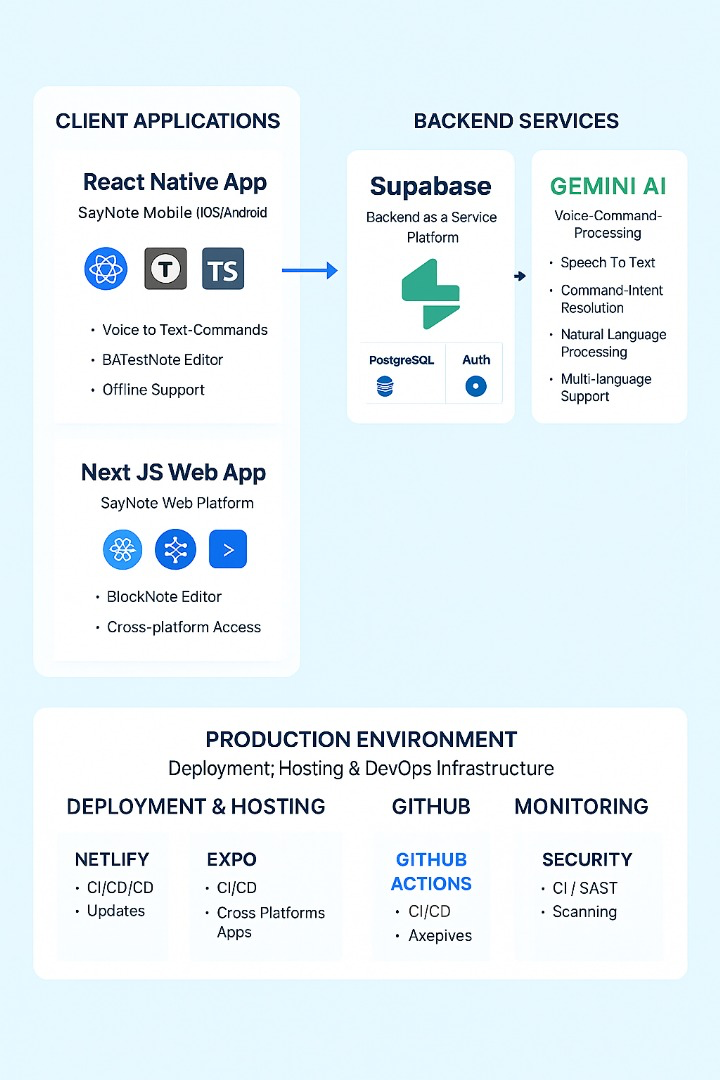
\includegraphics[width=0.8\textwidth]{assets/docs/global_architecture.png}
    \caption{Schéma d’architecture globale de SayNote}
    \label{fig:global-architecture}
\end{figure}

\section{Cas d’utilisation principaux}
SayNote répond à une variété de scénarios d’utilisation courants :
\begin{itemize}
    \item \textbf{Prise de notes en réunion :} Capturer rapidement les points clés, décisions et actions lors de réunions professionnelles ou associatives.
    \item \textbf{Notes d’étude :} Structurer des résumés de cours, fiches de révision et annotations pour les étudiants.
    \item \textbf{Saisie d’idées spontanées :} Enregistrer une idée, une inspiration ou une tâche à tout moment grâce à la saisie vocale instantanée.
    \item \textbf{Édition collaborative :} Partager et modifier des notes en temps réel avec d’autres utilisateurs pour faciliter le travail d’équipe.
    \item \textbf{Gestion de listes et d’organisateurs personnels :} Créer des listes de tâches, agendas ou carnets de bord personnalisés.
\end{itemize}

\section{Sécurité et confidentialité}
La sécurité et la confidentialité des données sont au cœur de la conception de SayNote :
\begin{itemize}
    \item \textbf{Authentification sécurisée :} Utilisation de Supabase pour une gestion robuste des comptes et des accès.
    \item \textbf{Chiffrement des données :} Les notes et informations sensibles sont stockées de manière chiffrée côté serveur.
    \item \textbf{Respect de la vie privée :} Aucune donnée personnelle n’est partagée avec des tiers sans consentement explicite.
    \item \textbf{Conformité RGPD :} Les utilisateurs peuvent exporter ou supprimer leurs données à tout moment, conformément aux exigences européennes.
\end{itemize}

\section{Accessibilité et inclusivité}
SayNote vise à offrir une expérience accessible à tous les utilisateurs :
\begin{itemize}
    \item \textbf{Commandes vocales avancées :} Navigation et édition complètes via la voix, réduisant la dépendance au clavier ou à l’écran tactile.
    \item \textbf{Mode hors-ligne :} Accès et modification des notes sans connexion internet, avec synchronisation automatique lors du retour en ligne.
    \item \textbf{Interface adaptable :} Thèmes clair/sombre, tailles de police ajustables et contrastes optimisés pour les personnes malvoyantes.
    \item \textbf{Compatibilité multi-appareils :} Utilisation fluide sur ordinateurs, tablettes et smartphones.
\end{itemize}

\section{Comparaison avec les solutions existantes}
Bien que des applications comme Notion ou Evernote proposent des fonctionnalités avancées, SayNote se distingue par :
\begin{itemize}
    \item \textbf{Intégration native de la saisie et édition vocale :} La voix est au centre de l’expérience, permettant une prise de notes plus rapide et naturelle.
    \item \textbf{Assistant IA embarqué :} Génération de résumés, réponses contextuelles et suggestions automatiques directement dans l’application.
    \item \textbf{Simplicité d’usage :} Interface épurée, prise en main rapide et fonctionnalités essentielles accessibles en un clic.
    \item \textbf{Synchronisation temps réel et mode hors-ligne complet :} Continuité de l’expérience utilisateur, même sans réseau.
\end{itemize}

\section{Limites actuelles et évolutions prévues}
Malgré ses atouts, SayNote présente certaines limites actuelles :
\begin{itemize}
    \item \textbf{Reconnaissance vocale perfectible :} La précision peut varier selon l’accent ou l’environnement sonore ; des améliorations sont prévues via l’intégration de nouveaux modèles.
    \item \textbf{Fonctionnalités collaboratives en développement :} Les options de coédition et de gestion avancée des partages seront enrichies dans les prochaines versions.
    \item \textbf{Personnalisation limitée :} De nouveaux thèmes, widgets et options de configuration sont à l’étude pour mieux répondre aux besoins variés des utilisateurs.
    \item \textbf{Intégrations tierces :} L’ajout de connecteurs avec d’autres outils (calendriers, gestion de tâches, etc.) est planifié.
\end{itemize}

\section*{Conclusion}
\addcontentsline{toc}{section}{Conclusion}
SayNote propose une solution innovante et complète pour la prise de notes moderne, alliant puissance technologique, simplicité d’utilisation et adaptabilité aux besoins des utilisateurs.
